\pdfoutput=1
%\documentclass[paper,twocolumn,twoside]{geophysics}
%\documentclass[manuscript]{geophysics}
\documentclass[manuscript,endfloat]{geophysics}
\usepackage{natbib}
\usepackage{graphicx}
\usepackage{amsmath}
\newcommand{\mitbf}[1]{\mathbf{{#1}}}

% To leave comments
\usepackage[colorinlistoftodos]{todonotes}

\title{
    Tesseroids: forward modeling gravitational fields in spherical coordinates
}
\author{
    Leonardo Uieda\footnotemark[1]\footnotemark[2],
    Val\'eria C. F. Barbosa\footnotemark[2],
    and
    Carla Braitenberg\footnotemark[3]
}


\begin{document}

\maketitle

\righthead{Tesseroids: modeling in spherical coordinates}
\ms{GEO-2015-0204} % manuscript number


\address{Peer-reviewed code related to this article can be found at
http://software.seg.org/2016/0004.
\\
\footnotemark[1]Universidade do Estado do Rio de Janeiro,
Rio de Janeiro, Brazil.
email: leouieda@gmail.com
\\
\footnotemark[2]Observat\'orio Nacional,
Rio de Janeiro, Brazil.
email: valcris@on.br
\\
\footnotemark[3]Department of Mathematics and Geosciences,
University of Trieste, Trieste, Italy
}

\begin{abstract}
We present the open-source software \emph{Tesseroids},
a set of command-line programs to perform the forward modeling
of gravitational fields in spherical coordinates.
The software is implemented in the C programming language and uses tesseroids
(spherical prisms) for the discretization of the subsurface mass distribution.
The gravitational fields of tesseroids are calculated numerically using
the Gauss-Legendre Quadrature (GLQ).
We have improved upon an adaptive discretization algorithm
to guarantee the accuracy of the GLQ integration.
Our implementation of adaptive discretization
uses a ``stack'' based algorithm
instead of recursion to achieve
more control over execution errors and corner cases.
The algorithm is controlled by
a scalar value called the distance-size ratio ($D$)
that determines the accuracy of the integration as well as
the computation time.
We determined optimal values of $D$
for the gravitational potential, gravitational acceleration,
and gravity gradient tensor
by comparing the computed tesseroids effects
with those of a homogeneous spherical shell.
The values required for a maximum relative error of 0.1\% of the shell effects
are $D = 1$ for the gravitational potential, $D = 1.5$ for the gravitational
acceleration, and $D = 8$ for the gravity gradients.
Contrary to previous assumptions,
our results show that the potential and its first and second derivatives
require different values of $D$ to achieve the same accuracy.
These values were incorporated as defaults in the software.
\end{abstract}



%%%%%%%%%%%%%%%%%%%%%%%%%%%%%%%%%%%%%%%%%%%%%%%%%%%%%%%%%%%%%%%%%%%%%%%%%%%%%%
\section{Introduction}


Satellite missions dedicated to measuring the Earth's gravity field
(like CHAMP, GRACE, and GOCE)
have provided geophysicists with almost uniform and global data coverage.
These new data have enabled interpretations on regional and global scales
\citep[e.g.][]{Reguzzoni2013,Braitenberg2015}.
Modeling at such scales requires taking into account the curvature of the
Earth and calculating gravity gradients as well as the traditional
gravitational acceleration.
A common approach to achieve this is
to discretize the Earth into tesseroids (Figure~\ref{fig:tesseroid})
instead of rectangular prisms.
An analytical solution exists when the computation point is along
the polar axis and the tesseroid is extended into a spherical cap
\citep{Lafehr1991, Mikuska2006, Grombein2013}.
For more general cases,
the integral formula for the gravitational effects of a tesseroid
must be solved numerically.
Approaches to this numerical integration include
Taylor series expansion \citep{Heck2007, Grombein2013}
and the Gauss-Legendre Quadrature \citep{Asgharzadeh2007}.
Taylor series expansion produces accurate results at low latitudes but
presents a decrease in accuracy towards the polar regions.
This is attributed to tesseroids degenerating into an approximately triangular
shape at the poles.
The Gauss-Legendre Quadrature (GLQ) integration consists in approximating
the volume integral by a weighted sum of the effect of point masses.
An advantage of the GLQ approach is that it can be
controlled by the number of point masses used.
The larger the number of point masses,
the better the accuracy of GLQ integration.
A disadvantage is the increased computation time as the number of
point masses increases.
Thus, there is a trade-off between accuracy and computation time.
This is a common theme in numerical methods.
\citet{Wild-Pfeiffer2008} investigated the use of different mass elements,
including tesseroids, to compute the gravitational effects of topographic
masses.
The author concludes that using tesseroids with GLQ integration gives the best
results for near-zone computations.
However, the question of how to determine the optimal parameters for GLQ
integration remained open.


Previous work by \citet{Ku1977} investigated the use of the GLQ
in gravity forward modeling.
\citet{Ku1977} numerically integrated the vertical component of the
gravitational acceleration of right rectangular prisms.
The author suggested that the accuracy of the GLQ integration depends on
the ratio between distance to the computation point and the distance between
adjacent point masses.
Based on this, \citet{Ku1977} proposed an empirical criterion that
the distance between point masses should be greater than
the distance to the computation point.
\citet{Asgharzadeh2007} used  this criterion for the GLQ integration of
the gravity gradient tensor of tesseroids.
To our knowledge, an analysis of how well this ad hoc criteria of
\citet{Ku1977} works for gravity gradient components or for tesseroids
has never been done before.
There has also been no attempt to quantify the error committed in the GLQ
integration when applying the criteria of \citet{Ku1977}.

\citet{Li2011} devised an algorithm to automatically enforce the criteria of
\citet{Ku1977}.
Their algorithm divides the tesseroid into smaller ones instead of increasing
the number of point masses per tesseroid.
A tesseroid is divided if the minimum distance to the computation point
is smaller than the largest dimension of the tesseroid.
This division is repeated recursively until all tesseroids obey the criterion.
Then, GLQ integration is performed for each of the smaller tesseroids
using the specified number of point masses.
The advantage of this adaptive discretization over
increasing the number of points masses is that the
total distribution of point masses will be greater
only close to the computation point.
This makes the adaptive discretization more computationally efficient.

\citet{Grombein2013} developed optimized formula for the gravitational fields
of tesseroids using Cartesian integral kernels.
These formulas are faster to compute and do not have singularities at the poles
like their spherical counterparts.
The Cartesian formulae are numerically integrated using a Taylor series
expansion as per \citet{Heck2007}.
\citet{Grombein2013} use a near-zone separation to mitigate the increased error
at high latitudes.
In the so called ``near-zone'' of the computation point they use a finer
discretization composed by smaller tesseroids.
This is accomplished by dividing the tesseroids along their horizontal
dimensions.
However, the determination of an optimal size of the near-zone remains an
open question \citep{Grombein2013}.

We have implemented a modified version of the adaptive discretion of
\citet{Li2011} into the open-source software package \emph{Tesseroids}.
The software uses the Cartesian formula of \citet{Grombein2013} for improved
performance and robustness.
Previous versions of the software have been used by, e.g.,
\citet{Alvarez2012, Bouman2013, Bouman2013a, Mariani2013, Braitenberg2014,
Braitenberg2011, Fullea2014}.

This article describes the software design and the implementation
of our modified adaptive discretization algorithm.
We also present a numerical investigation of the error committed
in the computations.
These results allow us to calibrate the adaptive discretization algorithm
separately for the gravitational potential, gravitational acceleration,
as well as the gravity gradient tensor components.


%%%%%%%%%%%%%%%%%%%%%%%%%%%%%%%%%%%%%%%%%%%%%%%%%%%%%%%%%%%%%%%%%%%%%%%%%%%%%%
\section{Theory}


\begin{figure}
    \centering
    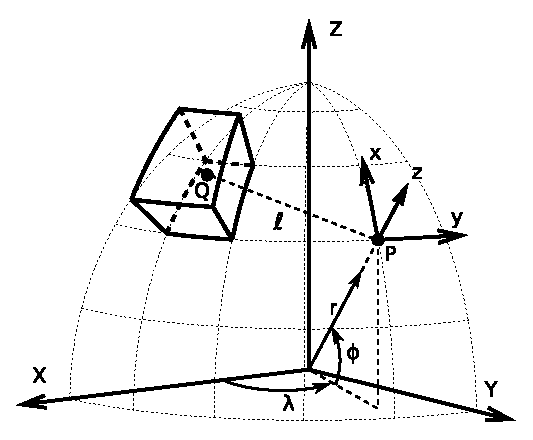
\includegraphics{figs/tesseroid}
    \caption{
        View of a tesseroid,
        the integration point $Q$ inside the tesseroid,
        a geocentric coordinate system $(X, Y, Z)$,
        the computation $P$ and it's local coordinate system $(x, y, z)$.
        $r$, $\phi$, $\lambda$ are
        the radius, latitude, and longitude, respectively, of point $P$,
        and $\ell$ is the Cartesian distance between $P$ and $Q$.
        After \citet{uieda2015}.
    }
    \label{fig:tesseroid}
\end{figure}

A tesseroid is a mass element defined in geocentric spherical
coordinates
(Figure~\ref{fig:tesseroid}).
It is bounded by two meridians, two parallels, and two concentric circles.
The gravitational fields of a tesseroid at a point $P = (r,\phi,\lambda)$
are determined with respect to the local North-oriented coordinate system at
P (x, y, z in Figure~\ref{fig:tesseroid}).
\citet{Grombein2013} formulated Cartesian kernels for the volume integrals
that define the tesseroid gravitational potential, gravitational acceleration,
and Marussi tensor, respectively,

\begin{equation}
    V(r,\phi,\lambda) = G \rho
        \int\limits_{\lambda_1}^{\lambda_2}
        \int\limits_{\phi_1}^{\phi_2}
        \int\limits_{r_1}^{r_2}
        \frac{1}{\ell}
        \kappa\  dr^\prime d\phi^\prime d\lambda^\prime,
    \label{eq:tesspot}
\end{equation}
\begin{equation}
    g_{\alpha}(r,\phi,\lambda) = G \rho
        \int\limits_{\lambda_1}^{\lambda_2}
        \int\limits_{\phi_1}^{\phi_2}
        \int\limits_{r_1}^{r_2}
        \frac{\Delta_\alpha}{\ell^3}
        \kappa\ dr^\prime d\phi^\prime d\lambda^\prime,
    \label{eq:tessgrav}
\end{equation}
\noindent
and
\begin{equation}
    g_{\alpha\beta}(r,\phi,\lambda) = G \rho
        \int\limits_{\lambda_1}^{\lambda_2}
        \int\limits_{\phi_1}^{\phi_2}
        \int\limits_{r_1}^{r_2}
        I_{\alpha\beta}
        \ \kappa\ dr^\prime d\phi^\prime d\lambda^\prime ,
    \label{eq:tesstensor}
\end{equation}
\begin{equation}
    I_{\alpha\beta} =
    \left(
        \frac{3\Delta_{\alpha} \Delta_{\beta}}{\ell^5} -
        \frac{\delta_{\alpha\beta}}{\ell^3}
    \right) ,
    \label{eq:tesstensorkernel}
\end{equation}

\noindent
where $\alpha, \beta \in \{x, y, z\}$,
$\rho$ is the density,
$G = 6.674\times10^{-11}\ m^3kg^{-1}s^{-1}$ is the gravitational constant,
$\delta_{\alpha\beta}$ is Kronecker's delta
($\delta_{\alpha\beta} = 1$ if $\alpha = \beta$
and $\delta_{\alpha\beta} = 0$ if $\alpha \neq \beta$),
and

\begin{equation}
    \Delta_x = r^\prime(\cos\phi\sin\phi^\prime - \sin\phi\cos\phi^\prime
               \cos(\lambda^\prime - \lambda)),
\end{equation}
\begin{equation}
    \Delta_y = r^\prime \cos \phi^\prime \sin(\lambda^\prime - \lambda),
\end{equation}
\begin{equation}
    \Delta_z = r^\prime \cos \psi - r,
\end{equation}
\begin{equation}
    \kappa = {r^\prime}^2 \cos \phi^\prime,
\end{equation}
\begin{equation}
    \ell = \sqrt{{r^\prime}^2 + r^2 - 2 r^\prime r \cos \psi},
\end{equation}
\begin{equation}
    \cos\psi = \sin\phi\sin\phi^\prime + \cos\phi\cos\phi^\prime
                 \cos(\lambda^\prime - \lambda).
\end{equation}

We will follow \citet{Asgharzadeh2007} and perform the numerical integration
using the Gauss-Legendre Quadrature (GLQ).
The GLQ consists in approximating the integral by a weighted sum of the
integration kernel \citep{Hildebrand1987},

\begin{equation}
    \int\limits_a^b f(x) dx \approx
    \frac{b-a}{2}\sum\limits_{i=1}^N W_i f(x_i),
    \label{eq:glq1d}
\end{equation}

\noindent
in which $N$ is the order of the quadrature,
i.e. the number of points used in the GLQ.
The points $x_i$ are called the quadrature nodes.
They are the roots of the $N^{th}$ order Legendre polynomial $P_N(x)$.
For a second order polynomial ($P_2(x)$),
the roots are $x = \pm 0.577350269$.
Roots for larger order polynomials
can be determined by a root finder algorithm.
Roots of Legendre polynomials
will be within the range $[-1, 1]$.
Before being used for GLQ integration,
the roots must be scaled to the integration limits $[a, b]$ using

\begin{equation}
    x^{scaled}_i = \frac{b - a}{2} x_i + \frac{b + a}{2}.
    \label{eq:glq_scaling}
\end{equation}

The weights of the GLQ are given by \citep{Hildebrand1987},

\begin{equation}
    W_i = \frac{2}{(1 - x_i^2)(P^\prime_N(x_i))^2}.
    \label{eq:glq_weights}
\end{equation}

\noindent
The values of $P_N(x)$ and its first derivative $P^\prime_N(x)$
can be calculated with recursive relations.

The Gauss-Legendre Quadrature for three-dimensional volume integrals,
like equations~\ref{eq:tesspot}-\ref{eq:tesstensor},
becomes \citep{Asgharzadeh2007}

\begin{equation}
    \iiint\limits_{\Omega}
    f(r^\prime, \lambda^\prime, \phi^\prime)
    d\Omega
    \approx
    A
    \sum\limits_{i=1}^{N^r}
    \sum\limits_{j=1}^{N^\phi}
    \sum\limits_{k=1}^{N^\lambda}
    W_i^r W_j^\phi W_k^\lambda
    f(r_i, \phi_j, \lambda_k),
    \label{eq:glq3d}
\end{equation}

\noindent
where

\begin{equation}
    A = \frac{(\lambda_2 - \lambda_1)(\phi_2 - \phi_1)(r_2 - r_1)}{8}.
\end{equation}

Comparing equation~\ref{eq:glq3d} with
equations~\ref{eq:tesspot}-\ref{eq:tesstensor},
we see that $f(r_i, \phi_j, \lambda_k)$ is the effect of a point
mass located on the quadrature nodes.
Thus, it can be said that the GLQ integration
approximates the volume integrals  by a
weighted sum of point mass effects.

The accuracy of the integration
depends on the number of point masses used in the summation.
\citet{Ku1977} showed that it also depends on the ratio between
the distance to the computation point and the distance between adjacent nodes.
Figure~\ref{fig:glqerrorsample}
illustrates this effect on the $g_{xy}$ gravity gradient component.
The $g_{xy}$ component was produced by a
$7^\circ \times 7^\circ \times 20\ km$ tesseroid
with $2.67\ g.cm^{-3}$ density
and top at $z=0\ km$.
The maps were calculated on a regular grid
with $100\times100$ points.
Figure~\ref{fig:glqerrorsample}a shows the $g_{xy}$ component
calculated at 400 km height using
GLQ with order two ($2 \times 2 \times 2 = 8$ point masses).
Figure~\ref{fig:glqerrorsample}b shows $g_{xy}$ computed with order two
GLQ as well but at 150 km height.
Notice that the computed effect is concentrated around each point mass
of the GLQ (black dots) and does not resemble the effect of a tesseroid.
\citet{Ku1977} determined an ad hoc criterion that the distance between
point masses (quadrature nodes) should be smaller than the minimum distance to
the computation point.
Thus, if a computation point is too close to the tesseroid one would have to
decrease the distance between the point masses in order to obtain an accurate
result.
One way to accomplish this would be increase the order of the quadrature
$N$ in all three directions.
Figure~\ref{fig:glqerrorsample}c shows the $g_{xy}$ component calculated at
150km height but with a GLQ order of 30
($30 \times 30 \times 30 = 27,000$ point masses).
The computed $g_{xy}$ component more closely resembles
the expect results for a single tesseroid \citep{Asgharzadeh2007}.

\begin{figure}
    \centering
    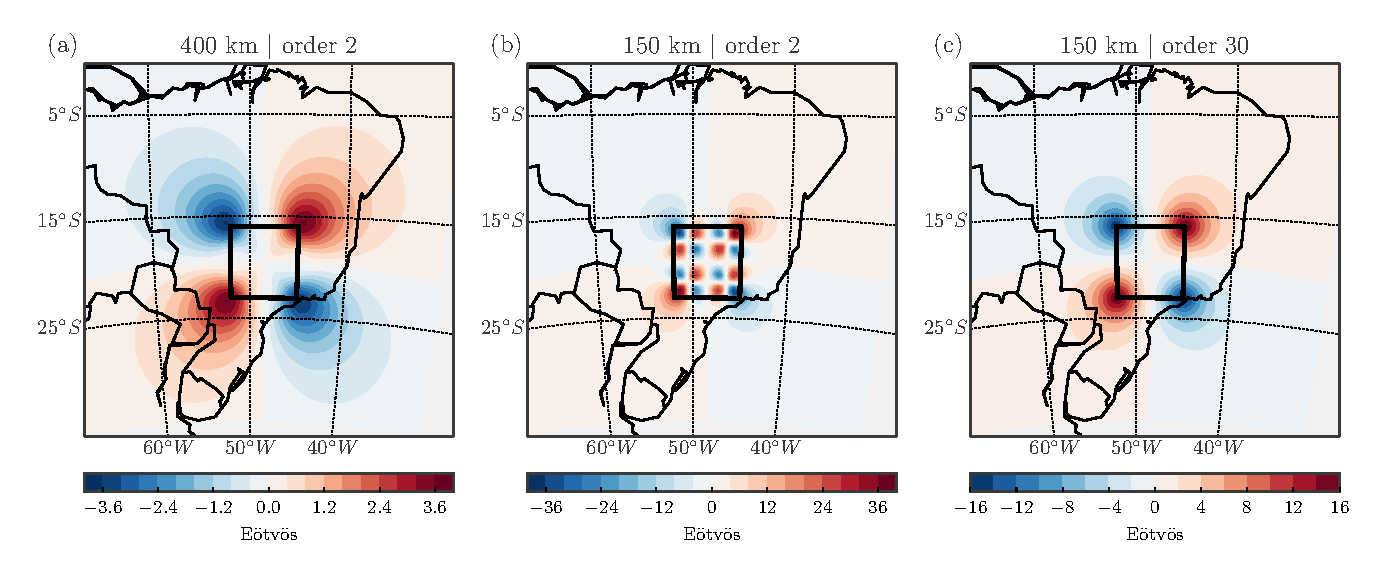
\includegraphics[width=0.4\textwidth]{figs/vary-height-and-order}
    \caption{
        Example of the effect of varying
        the computation height
        and the number of point masses in the Gauss-Legendre Quadrature.
        Black circles represent the horizontal location of the point masses.
        a) $g_{xy}$ calculated at $400\ km$ height using GLQ order 2
        ($2 \times 2 \times 2 = 8$ point masses).
        b) At $150\ km$ height and GLQ order 2,
        the result resembles that of
        four point masses instead of a single tesseroid.
        This effect was shown by \citet{Ku1977}.
        c) At $150\ km$ but with a higher GLQ order of 30.
        In (c) the horizontal locations of the point masses were not shown.
        Notice that the results shown in (c) are similar to that expected
        for a single mass source.
    }
    \label{fig:glqerrorsample}
\end{figure}


\subsection{Adaptive discretization}

\citet{Li2011} proposed an alternative method
for decreasing the distance between point masses on the quadrature nodes
aiming at achieving an accurate integration.
Instead of increasing the GLQ order,
they keep it fixed to a given number
and divide the tesseroid into smaller volumes.
The sum of the effects of the smaller tesseroids
is equal to the gravitational effect of the larger tesseroid.
This division effectively decreases
the distance between nodes because
of the smaller size of the tesseroids.
The criterion for dividing a tesseroid is that the distance to the computation point
should be smaller than a constant times the size of the tesseroid.
This is analogous to the criterion proposed by \citet{Ku1977}
because the size of the tesseroid serves as a proxy
for the distance between point masses.
This procedure is repeated recursively
until all tesseroids are within the acceptable
ratio of distance and size or a minimum size is achieved.

The advantage of this adaptive discretization is
that the number of point masses is only increased
in parts of the tesseroid that are
closer to the computation point.
Notice that the alternative approach of
simply increasing the order of the GLQ
would increase the number of point masses
evenly throughout the whole tesseroid.


%%%%%%%%%%%%%%%%%%%%%%%%%%%%%%%%%%%%%%%%%%%%%%%%%%%%%%%%%%%%%%%%%%%%%%%%%%%%%%
\section{Implementation}

We have implemented the calculation of
the tesseroid gravitational fields
with adaptive discretization
in version 1.2 of the open-source package \emph{Tesseroids}.
It is freely available online\footnote{
http://tesseroids.leouieda.com}\footnote{
http://dx.doi.org/10.5281/zenodo.16033}
under the BSD 3-clause open-source license.
An archived version of the source code
is also available as part of this article.

\emph{Tesseroids} consists of command-line programs
written in the C programming language.
The package includes programs to calculate
the gravitational fields of tesseroids and
rectangular prisms (in both Cartesian and spherical coordinates).
All programs receive input through
command-line arguments and the standard input channel (``STDIN'')
and output the results through the standard output channel (``STDOUT'').
For example,
the command to generate a regular grid with $NLON \times NLAT$ points,
 calculate $g_z$ and $g_{zz}$ caused by
the tesseroids in a file ``MODELFILE'',
and save the results to a file called ``OUTPUT''
is:

\begin{verbatim}
tessgrd -rW/E/S/N -bNLON/NLAT -zHEIGHT | \
    tessgz MODELFILE | \
    tessgzz MODELFILE > OUTPUT
\end{verbatim}

The \emph{src} folder of the source code archive
contains the C files that build the command-line programs
(e.g., \emph{tessgz.c}).
The \emph{src/lib} folder contains
the source files that implement the numerical computations.
We will not describe here the implementation of the input/output parsing and
other miscellanea.
Instead, we will focus on the details of the Gauss-Legendre Quadrature
integration of equations~\ref{eq:tesspot}-\ref{eq:tesstensor}
and the adaptive discretization of tesseroids.



\subsection{Numerical integration}

The source file \emph{src/lib/glq.c}
contains the code necessary to perform
a Gauss-Legendre Quadrature integration.
The first step in the GLQ is to compute the
locations of the discretization points (i.e., the point masses).
These points are roots of Legendre polynomials.
Precomputed values are available for low order polynomials,
typically up to order five.
For flexibility and to compute higher order roots,
we use the multiple root-finder algorithm of
\citet{Barrera-Figueroa2006}.
The additional computational load is minimal
because the root-finder algorithm
must be run only once per program execution.
The root-finder is implemented in functions
\emph{glq\_nodes} and \emph{glq\_next\_root}.
The computed roots will be in the range $[-1, 1]$
and must be scaled to the integration limits
(the physical boundaries of the tesseroid)
using function \emph{glq\_set\_limits} (see equation~\ref{eq:glq_scaling}).

The GLQ weights (equation~\ref{eq:glq_weights})
are computed by function \emph{glq\_weights}.
Both the computed roots and weights are stored in a data structure
(a C \emph{struct}) called \emph{GLQ}.
Function \emph{glq\_new}
handles memory allocation,
calculates the roots and weights,
and returns the complete \emph{GLQ} structure.

The numerical integration of the tesseroid gravitational fields
is performed by the functions in module \emph{src/lib/grav\_tess.c}.
Functions \emph{tess\_pot}, \emph{tess\_gx}, \emph{tess\_gy}, and so on,
compute the gravitational fields of a single tesseroid
on a single computation point.
These functions require three \emph{GLQ} structures,
each containing the roots and weights
for GLQ integration in the three dimensions.
The roots must be scaled to the
integration limits
$[\lambda_1, \lambda_2], [\phi_1, \phi_2], [r_1, r_2]$
(see equations~\ref{eq:tesspot}-\ref{eq:tesstensor}).
The integration consists of three loops
that sum the weighted kernel functions
evaluated at each GLQ point mass (the scaled roots).

The biggest bottlenecks for the numerical integration are
the number of point masses used
and the evaluation of the trigonometric functions in
equations~\ref{eq:tesspot}-\ref{eq:tesstensor} inside the inner loops.
Better performance is achieved
by pre-computing the sine and cosine of latitudes
and moving some trigonometric function evaluations
to the outer loops.


\subsection{Implementation of adaptive discretization}

Our implementation of the adaptive discretization algorithm
differs in a few ways from the one proposed by \citet{Li2011}.
In \citet{Li2011},
a tesseroid will be divided when
the smallest distance between it and the computation point
is smaller than a constant times
the largest dimension of the tesseroid.
Instead of the smallest distance,
we use the easier to calculate
distance between
the computation point $(r, \lambda, \phi)$
and the geometric center of the tesseroid
$(r_t, \lambda_t, \phi_t)$

\begin{equation}
    d = \left[
        r^2 + r_t^2 - 2 r r_t \cos\psi_t
        \right]^{\frac{1}{2}} ,
    \label{eq:distance}
\end{equation}
\begin{equation}
    \cos\psi_t =
        \sin\phi\sin\phi_t + \cos\phi\cos\phi_t\cos(\lambda - \lambda_t) .
\end{equation}

Our definition of the dimensions of the tesseroid
(the ``side lengths'' of \citet{Li2011})
along longitude, latitude, and radius, respectively, are
(Figure~\ref{fig:division}a)

\begin{equation}
    L_\lambda = r_2 \arccos(\sin^2\phi_t +
        \cos^2\phi_t\cos(\lambda_2 - \lambda_1)),
    \label{eq:sizelon}
\end{equation}
\begin{equation}
    L_\phi = r_2 \arccos(\sin\phi_2\sin\phi_1 + \cos\phi_2\cos\phi_1),
\end{equation}
\begin{equation}
    L_r = r_2 - r_1.
    \label{eq:sizer}
\end{equation}

\noindent
$L_\lambda$ and $L_\phi$ are arc-distances measured along the top surface of
the tesseroid (Figure~\ref{fig:division}a).
Specifically, $L_\lambda$ is measured long the middle latitude of the
tesseroid ($\phi_t$).

To determine if a tesseroid must be divided,
we check if

\begin{equation}
    \frac{d}{L_i} \geq D,
    \label{eq:condition}
\end{equation}

\noindent
for each $i \in (\lambda, \phi, r)$.
$D$ is a positive scalar
hereafter referred to as the ``distance-size ratio''.
If the inequality holds for all three dimensions,
the tesseroid is not divided.
Thus, the distance-size ratio determines
how close the computation point can be
before we must divide the tesseroid.
The value of $D$ is indirectly responsible for
the accuracy of the solution and the computation time.
We will explore the relationship with the accuracy in the following section.

Figure~\ref{fig:division} shows examples of
the resulting tesseroid models after adaptive discretization.
Figure~\ref{fig:division}a shows
the initial tesseroid and computation point P.
Figures~\ref{fig:division}b-d are
the result of adaptive discretization using
different values of the distance-size ratio $D$,
respectively,
$D=1$, $D=2$, and $D=6$.
The number of tesseroids in the resulting discretization is, respectively,
4, 38, and 936.

\begin{figure}
    \centering
    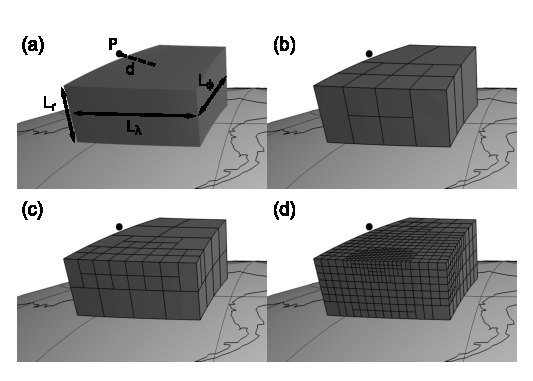
\includegraphics{figs/tesseroid-split}
    \caption{
        Adaptive discretization
        of the tesseroid shown in (a)
        for a computation point P
        using the distance-size ratio $D$ equal to
        (b) 1, (c) 2, and (d) 6.
        $L_r$, $L_\phi$, and $L_\lambda$ are the dimensions of the tesseroid.
        Note that increasing $D$
        results in a fine division of the tesseroid
        close the computation point
        and a coarser division further away.
    }
    \label{fig:division}
\end{figure}

Instead of using recursive function calls,
as originally proposed by \citet{Li2011},
we use a stack-based implementation of the algorithm.
Stacks are array-like data structures
with a particular way of inserting and removing elements from it.
In a stack,
one can only insert elements to the top of the stack
(the last empty position).
Likewise,
one can only remove the last element of the stack
(commonly referred to as ``popping'' the stack).
Because of these restrictions,
stacks are also known as ``Last-In-First-Out'' (LIFO) data structures.

The discretization algorithm is implemented in
function \emph{calc\_tess\_model\_adapt}
of the file \emph{src/lib/grav\_tess.c}.
This function calculates the effect of a single tesseroid
on a single computation point.
The stack of tesseroids is represented by
the \emph{stack} variable,
an array of \emph{TESSEROID} structures.
We must define a maximum size for the stack to allocate memory for it.
Defining a maximum size allows us to
avoid an infinite loop
in case the computation point is on
(or sufficiently close to) the surface of the tesseroid.
We use the integer \emph{stktop}
to keep track of the index of
the last element in the stack (the top of the stack).

Below, we describe the algorithm to calculate
the effect of a single tesseroid from the input model
on a single computation point.
The algorithm starts by creating an empty stack of tesseroids.
Then, the stack is initialized with the single input tesseroid.
The initialization is done by copying the tesseroid into the stack
and setting \emph{stktop} to zero (the first element).
It is important to note that the stack is not the input tesseroid model.
Instead, it is a buffer used to temporarily store
each stage of the discretization algorithm.

Once the stack is initialized, the steps of the algorithm are:

\begin{enumerate}
    \item ``Pop'' the stack (i.e., take the last tesseroid from it).
        This will cause \emph{stktop} to be reduced by one.
        This tesseroid is the one that will be evaluated in the following
        steps.
    \item Compute the distance $d$ (equation~\ref{eq:distance}) between
        the geometric center of the tesseroid and
        the computation point.
    \item Compute the dimensions of the tesseroid $L_\lambda$, $L_\phi$,
        and $L_r$ using equations~\ref{eq:sizelon}-\ref{eq:sizer}.
    \item Check the condition in equation~\ref{eq:condition} for each
        dimension of the tesseroid.
    \item If all dimensions hold the inequality \ref{eq:condition},
        the tesseroid is not divided and its
        gravitational effect is computed using the
        Gauss-Legendre Quadrature
        (equations~\ref{eq:tesspot}-\ref{eq:tesstensor} and~\ref{eq:glq3d}).
        We use a GLQ order of two for all three dimensions
        ($2 \times 2 \times 2 = 8$ point masses)
        by default.
        This value can be changed using
        a command-line argument of the modeling programs.
    \item If any of the dimensions fail the condition:
    \begin{enumerate}
        \item Divide the tesseroid in half along each dimension that failed
             the condition.
        \item Check if there is room in the stack
            for the new tesseroids
            (i.e.,the number of new elements plus \emph{stktop}
             is smaller than the maximum stack size).
             If there isn't,
             warn the user of a ``stack overflow''
             and compute the effect of the tesseroid, as in step 5.
             If there is room in the stack,
             place the smaller tesseroids into
             the stack.
    \end{enumerate}
    \item Repeat the above steps until the stack is empty
        (\emph{stktop} is equal to -1).
\end{enumerate}

The algorithm above is repeated
for every tesseroid of the input model
and the results are summed.
This will yield the gravitational effect
of the input tesseroid model on a single point.
Thus, the computations must be repeated
for every computation point.
The whole algorithm can be summarized
in the following pseudo-code.

\begin{verbatim}
Initialize the output array with zeros.
for tesseroid in model:
  for point in grid:
    Initialize the stack with tesseroid.
    stktop = 0
    while stktop >= 0:
      Perform steps 1-6 of the algorithm.
    Sum the calculated value to the output.
\end{verbatim}

This stack-based implementation
has some advantages over the original recursive implementation,
namely:
(1) It gives the developer more control over the recursion step.
(2) In general, it is faster because it bypasses the overhead of function
calls.
In recursive implementations,
the developer has no control over
the maximum number of consecutive recursive calls
(i.e., the ``recursion depth'').
This limit may vary with programming language,
compiler, and operating system.
Overflowing the maximum recursion depth
may result in program crashes,
typically with cryptic or inexistent error messages.
In the stack-based implementation,
the developer has complete control.
Overflowing of the stack can be handled gracefully
with an error message
or even performing a suitable approximation of the result.

\subsection{Code for figures and error analysis}


The error analysis and all figures in this article
were produced in IPython notebooks
\citep{Perez2007}.
The notebook files combine source code in various programming languages,
program execution,
text, equations,
and the figures generated by the code
into a single document.
We used the following Python language libraries
to perform the error analysis and generate figures:
\emph{pandas} by \citet{Mckinney2010},
\emph{matplotlib} by \citet{Hunter2007} for 2D figures and maps,
and \emph{Mayavi} by \citet{Ramachandran2011} for 3D figures.

The IPython notebooks
and the data generated for the error analysis,
as well as instructions for installing the software
and running the programs,
are also included in
the source code archive that accompanies this article.
Alternatively,
all accompanying material is available
in an online repository\footnote{
https://github.com/pinga-lab/paper-tesseroids}.



%%%%%%%%%%%%%%%%%%%%%%%%%%%%%%%%%%%%%%%%%%%%%%%%%%%%%%%%%%%%%%%%%%%%%%%%%%%%%%
\section{Evaluation of the accuracy}



The key controlling point of the adaptive discretization algorithm
is the distance-size ratio $D$ (equation~\ref{eq:condition}).
The specific value chosen for $D$ determines how many divisions will be made
(Figure~\ref{fig:division}).
Thus, $D$ indirectly controls both the accuracy of the integration
and the computation time.
In this section, we investigate the relationship between
the distance-size ratio and the integration error.
We perform the analysis for the gravitational potential,
acceleration, and gradient tensor components
to evaluate if the same value of $D$ yields compatible error levels
for different fields.

The reference against which we compare the computed tesseroid fields
is a homogeneous spherical shell.
The shell has analytical solutions along the polar axis
\citep{Lafehr1991, Mikuska2006, Grombein2013}
and can be perfectly discretized into tesseroids.
We chose a spherical shell with a thickness of 1 km,
density of $2670\ kg.m^{-3}$,
bottom at height 0 km above the reference sphere,
and top at 1 km height.
We produced tesseroid models of the shell by discretizing it along the
horizontal dimensions into a regular mesh.


Figure~\ref{fig:glqerrorsample} shows that the largest errors are spread over
on top of the tesseroid.
Thus, calculating the tesseroid fields at a single point might not
capture the point of largest error.
Instead, we calculate the effect of the tesseroid model on a regular grid
of $10 \times 10$ points at different geographic locations
(see Table~\ref{tbl:experiment}).
Fortunately, the symmetry of the shell allows us to consider the computation
point at any geocentric coordinate.
Therefore, the effect of the shell will be same along the entire grid.
We compute the differences between the effects of the shell and the tesseroid
model on the grid.
However, we will consider only the largest error in our analysis.


We placed the grid on top of a particular tesseroid
to increase the chances of capturing the true largest integration error.
We calculate the errors for values of the distance-size ratio
$D$ varying from 0 (i.e., no divisions) to 10 in 0.5 intervals.
Furthermore, we repeated the error analysis in four different numerical experiments,
each with computation grids at different locations and
different tesseroid model sizes.
Table~\ref{tbl:experiment} describes the different numerical
experiments and the corresponding parameters of the computation grid and
tesseroid model.


Figure~\ref{fig:dist-size-curves} shows
the maximum difference between the shell and tesseroid fields
as a function of $D$ for the four experiments.
The differences are given as a percentage of the shell value.
We established a maximum tolerated error of $0.1\%$, represented by the
horizontal solid lines in Figure~\ref{fig:dist-size-curves}.
Only results for the gravitational potential, $g_z$, and $g_{zz}$ are shown.
The results for the other diagonal components of the gravity gradient tensor
are similar to $g_{zz}$.
Figures for these components can be found in the supplementary material
(see section "Reproducing the analysis and results").


For the potential $V$, a distance-size ratio $D=1$ guarantees that the curves
for all experiments are below the $0.1\%$ error threshold.
For $g_z$, the same is achieved with $D=1.5$.
Conversely, $g_{zz}$ requires a value of $D=8$ to achieve an error level of
$0.1\%$.
For a computation height of 260 km, the error curve for $g_{zz}$
intercepts the error threshold line at $D=2.5$.
This behavior suggests that the error curves for $g_{zz}$ might depend on the
computation height.
To test this hypothesis, we computed the error curves for $g_{zz}$ at
heights 2, 10, 50, 150, and 260 km.
Figure~\ref{fig:gzz-with-height} shows the results for $g_{zz}$ at varying
computation heights.
Notice that the distance-size ratio required to achieve $0.1\%$ accuracy
decreases as the computation height increases.
For example, computation at 260 km height requires $D=2.5$ whereas at 10 km
height a value of $D=5.5$ is required to achieve the same accuracy.
One can take advantage of this behavior to reduce the distance-size ratio for
computations of the gravity gradient tensor at high altitudes,
saving computation time.


We have implemented the values of the distance-size ratio producing $0.1\%$
accuracy determined above as defaults for the software \emph{Tesseroids}.
We chose the conservative value of $D=8$ for the gravity gradient components
as a fail-safe alternative.
Users can control the value of $D$ used in the computations through
command-line arguments to achieve greater performance at the cost of
accuracy.


\begin{table*}
\centering
\begin{tabular}{lccc}
    \hline
    ~             & Grid location & Grid height & Tesseroid size \\
    \hline
    Experiment 1 (pole)            & 89N--90N/0E--1E  & 2 km   & $1^\circ \times 1^\circ$ \\
    Experiment 2 (equator)         & 0N--1N/0E--1E    & 2 km   & $1^\circ \times 1^\circ$ \\
    Experiment 3 (260 km)          & 89N--90N/0E--1E  & 260 km & $1^\circ \times 1^\circ$ \\
    Experiment 4 ($30^\circ$ size) & 60N--90N/0E--30E & 2 km   & $30^\circ \times 30^\circ$ \\
    \hline
\end{tabular}
\caption{
    Parameters of the numerical experiments to quantify the accuracy of
    the numerical integration.
    All grids had $10\times10$ regularly spaced computation points at a
    constant height.
    Tesseroids used to discretize the spherical shell had 1 km thickness and
    the horizontal dimensions shown in the table.
}
\label{tbl:experiment}
\end{table*}



\begin{figure}
    \centering
    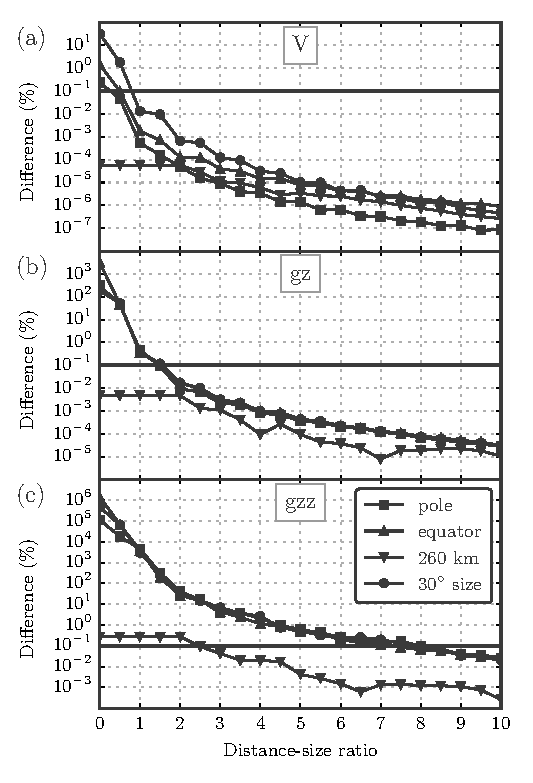
\includegraphics{figs/distance-size-curves}
    \caption{
        The maximum difference between the computed tesseroid and shell effects
        as a function of the distance-size ratio $D$
        for (a) the gravitational potential, (b) $g_z$, and (c) $g_{zz}$.
        The difference is given as a percentage of the shell effect.
        Curves correspond to the different tesseroid models and computation
        grids shown in Table~\ref{tbl:experiment}.
        The horizontal solid black line marks the established error threshold
        of $0.1\%$.
        A value of $D=0$ means that no divisions are made.
    }
    \label{fig:dist-size-curves}
\end{figure}

\begin{figure}
    \centering
    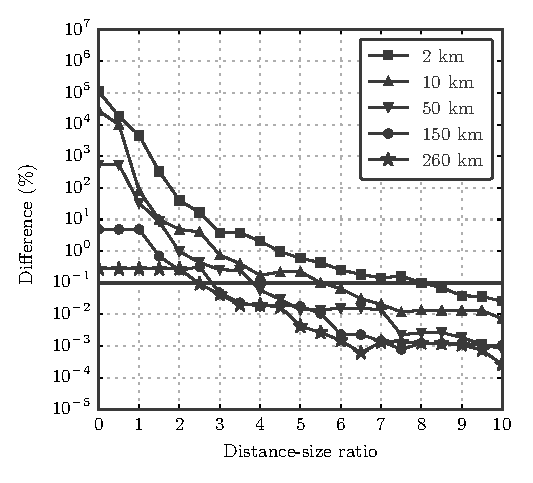
\includegraphics{figs/gzz-with-height}
    \caption{
        Difference between the computed $g_{zz}$ for the spherical shell and
        the tesseroid model at different heights. Curves show the maximum
        difference as a percentage of the shell value.
        The horizontal solid black line marks the established error threshold
        of $0.1\%$.
        A value of $D=0$ means that no divisions are made.
    }
    \label{fig:gzz-with-height}
\end{figure}


%%%%%%%%%%%%%%%%%%%%%%%%%%%%%%%%%%%%%%%%%%%%%%%%%%%%%%%%%%%%%%%%%%%%%%%%%%%%%%
\section{Conclusions}


We have presented the open-source software \emph{Tesseroids}.
It consists of command-line programs,
written in the C programming language,
to perform the forward modeling of gravitational fields in spherical
coordinates.
The fields are calculated from a mass model composed of spherical prisms, the
so-called tesseroids.
The volume integrals of the gravitational fields of a tesseroid are solved
numerically using the Gauss-Legendre Quadrature (GLQ).
The GLQ approximates the volume integrals by weighted sums of point mass
effects.
The error of the GLQ integration increases as the computation point gets closer
to the tesseroid.
To counter this effect,
the accuracy of the GLQ integration can be increased by using more point
masses or by dividing each tesseroid into smaller ones.


We have implemented and improved upon an adaptive discretization algorithm to
achieve an optimal division of tesseroids.
Tesseroids are divided into more parts closer to the computation point,
where more point masses are needed.
Our implementation of the adaptive discretization uses a ``stack'' data
structure in place of the originally proposed recursive implementation.
As a rule of thumb in procedural languages (like C),
stack-base implementations are computationally faster
than the equivalent code using function recursion.
Furthermore, the stack-based algorithm allows more control
over errors when too many divisions are necessary.
The adaptive discretization is controlled by
a scalar called the distance-size ratio ($D$).
The algorithm ensures that all tesseroids will
have dimensions smaller than $D$ times the distance to the computation point.
The value of $D$ indirectly controls the accuracy of the integration as well as
the computation time.


We performed an error analysis to determine
the optimal value of $D$ required to achieve a target accuracy.
We used a spherical shell as a reference to calculate the computation error of
our algorithm for different values of $D$.
Our results show that the values of $D$ required to achieve a maximum error
of 0.1\% of the shell values are
1 for the gravitational potential, 1.5 for the gravitational acceleration,
and 8 for the gravity gradients.
Previous assumptions in the literature
were that accurate results are guaranteed if
the distance to the tesseroid is larger than
the distance between point masses.
This condition was previously applied indiscriminately
to both the gravitational acceleration and the gravity gradients.
That assumption is equivalent to using $D=1.5$ for all fields.
Our results show that this is valid for the gravitational
acceleration and results in a 0.1\% computation error.
This is expected because the original study that determined the above condition
was performed on the vertical component of gravitational acceleration.
However, applying the same condition to the gravity gradients produces
an error of the order of $10^2\%$.


For the gravity gradients in particular,
the distance-size ratio required for 0.1\% error decreases with height.
We believe this is because the decay factor for
the gravity gradient components is $d^{-3}$,
whereas the discretization algorithm uses $d/L_i$.
As the computation point becomes closer to the tesseroid,
the field increases more rapidly than
the algorithm increases the amount of discretization.
Hence, a higher value of D (i.e., more discretization)
is required.


The values of the distance-size ratio determined above were
incorporated as defaults in the software \emph{Tesseroids}.
We chose the value $D=8$ for the gravity gradients as a conservative default.
If the user desires, the value of $D$ used can be controlled by a command-line
argument.


In situations that require many tesseroid divisions,
the stack used in the algorithm will overflow and further
divisions become impossible.
The current implementation warns the user that
the overflow occurred and proceeds with the GLQ integration without division.
Future improvements to the algorithm include a better way to handle such
situations as they arise.
An alternative would be to replace the tesseroid by an equivalent
right rectangular prism and compute its effects instead.
This would allow accurate computations at smaller distances.
Furthermore,
the computation time increases drastically as the computation point
gets closer to the tesseroid.
This effect can be prohibitive for computing the gravity gradients at
relatively low heights (e.g., for terrain corrections of
ground or airborne surveys).
Further investigation of different criteria for dividing the tesseroids could
yield better performance through a reduced number of divisions.


%%%%%%%%%%%%%%%%%%%%%%%%%%%%%%%%%%%%%%%%%%%%%%%%%%%%%%%%%%%%%%%%%%%%%%%%%%%%%%
\section{Acknowledgments}

The authors were supported in this research by
a fellowship (VCFB) from
Conselho Nacional de Desenvolvimento Cient\'ifico e Tecnol\'ogico (CNPq)
and a scholarship (LU) from
Coordena\c{c}\~ao de Aperfei\c{c}oamento de Pessoal de N\'ivel Superior
(CAPES),
Brazil.
Additional support for the authors was provided by
the Brazilian agency FAPERJ (grant E-26/103.175/2011)
and by the GOCE-Italy project (ASI).

\bibliographystyle{seg}
\bibliography{references.bib}
\end{document}
